	The Fraunhofer-Institut f\"ur Produktionstechnologie, in Aachen, Germany, develops systems and solutions for production. It focuses on the topics of process technology, production machines, mechatronics, production quality and metrology as well as technology management.

	Its clients and cooperation partners represent all fields of industry: from aerospace technology to the automotive industry and its suppliers as well as tool and die making companies and the precision mechanics, optics and machine tool industries in particular.
	
	The "Fine machining \& optics" department is part of the Process technology competence. It develops technologies for the production and processing of high-precision components including glass lenses, replication tools and components for the semi-conductor industry. The technology portfolio includes the ultra-precise grinding and polishing, diamond machining and precision molding.
	
	The "Ultra-Precision Technology and Polymer Replication" group, is a sub department of the "Fine machining \& optics". This team forms high-precision polymer optics using the injection molding technique as well as directly machining optics from polymers and mold inserts via ultra-precision processes. The development activities take the entire process into account, from the material selection, the ultra-precision machining of the mold using single crystal diamond tools, the application of the mold for mold injection replication processes, the machining of prototypes on plastic, all the software operations in between phases and within the phases themselves, among other processes.
	
	This group uses a proprietary software, called LODTa -- Light Optimal Distribution Tool (alpha) --, which was developed by another institute, the Fraunhofer-Institut f\"ur Techno- und Wirtschatftsmathematik, in Kaiserslautern, Germany. It uses geometrical optics theory to calculate the freeform surface necessary for a lens to project a monochromatic image onto a screen using a given light source. It takes as input the following information:
	\newpage
	
	\begin{itemize}
		\item Black and white square image file for the image to be projected;
		\item Size of desired projection;
		\item Lens material and refraction index;
		\item Lens diameter and thickness;
		\item Type of light source (point source, sunlight, etc);
		\item Distance between light source and lens;
		\item Distance between lens and projection screen.
	\end{itemize}
	
	With this information, the software calculates the geometry of the lens surface.
	
	\begin{figure}[H]
		\centering
		\captionsetup{justification=centering}
		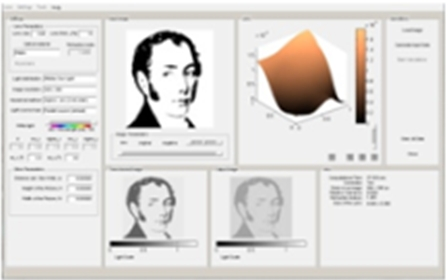
\includegraphics[width=0.9\linewidth]{Cap2/LODTa/lodta_screenshot.jpg}
		\caption{LODTa software for lens surface calculation.}
		\label{fig:lodta_screenshot}
	\end{figure}
	
	The software then generates an IGES file which contains the calculated lens geometry. It is generated as a square piece, from which the round lens will be extracted. This surface is completed with 5 other plane surfaces, forming a closed volume, as shown in Figure~\ref{fig:lodta_iges}. One of its vertexes is positioned on the origin of the XY-plane, and it occupies the quadrant I of the plane. Therefore, it can be centered by shifting half of its size in the negative X direction and in the negative Y direction.
	
	\begin{figure}[H]
		\centering
		\captionsetup{justification=centering}
		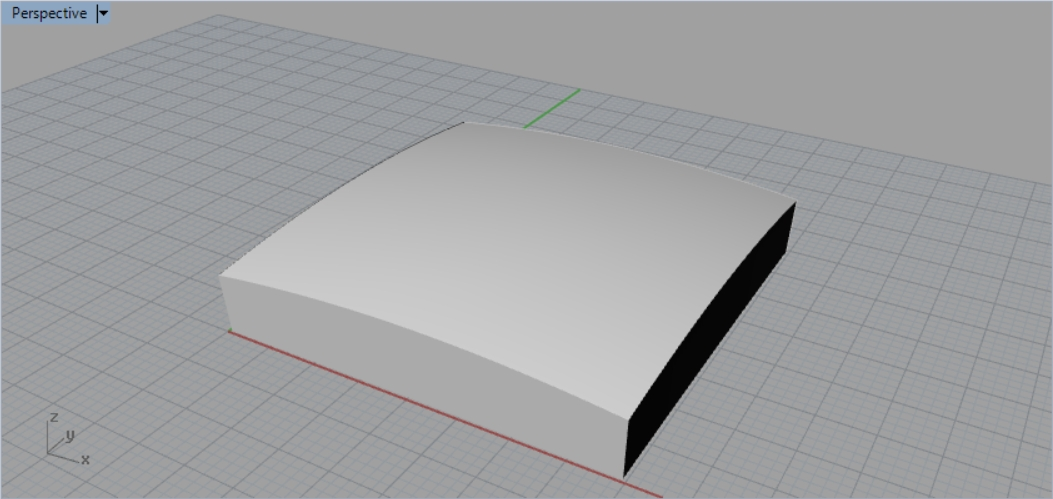
\includegraphics[width=\linewidth]{Cap2/LODTa/lodta_iges.jpg}
		\caption{Visualization of IGES file generated by LODTa. Screenshot from Rhinoceros 5.}
		\label{fig:lodta_iges}
	\end{figure}